

\documentclass[11pt,addpoints,letterpaper]{exam}
\usepackage{amsmath,tcolorbox,mdframed,xcolor}
\usepackage[top=0.75in, bottom=0.85in, left=1in, right=1in]{geometry} % Adjust margins
\usepackage{mathtools}
\usepackage{siunitx}
\usepackage{nccmath}
\usepackage{physics}
\usepackage{tikz}
\usepackage{multicol}
\usepackage{epigraph}
\usepackage{cancel}
\usepackage{xfrac}
\usepackage{pgfplots}
\usepackage{array}   % For alignment
\usepackage{booktabs} % For better horizontal lines
\usepackage{caption} % For caption formatting
\usepackage{graphicx} % For scaling tables if needed

\setlength\epigraphwidth{.8\textwidth}
\setlength\epigraphrule{0pt}

\noprintanswers

\newcommand{\Section}[1]{
\textbf{\\\Large #1\\}
}
\newcommand{\labheader}[4]{%
  \vspace*{-0.2in} % Adjust vertical spacing
  \noindent
  \makebox[0.65\textwidth][l]{Name:\enspace\hrulefill\,\,\,}
  \makebox[0.1\textwidth][l]{\,Period:\enspace}
  \makebox[0.25\textwidth][l]{\hrulefill}\\[0.25cm]
  \makebox[0.65\textwidth][l]{Instructor: \enspace\texttt{\underline{#1}}}\hfill
  \makebox[0.1\textwidth][l]{ Course: }\hfill 
  \makebox[0.25\textwidth][l]{ \texttt{\underline{#2}}}\hfill \\[0.25cm]
  \makebox[0.65\textwidth]{}\makebox[0.1\textwidth][l]{ Term: }\hfill
  \makebox[0.25\textwidth][l]{\enspace\texttt{\underline{#3}}}\hfill
  \hfill{Score: \underline{\hspace{2cm}}/#4}
  \vspace{0.5in}
}

% Define variables
\newcommand{\instructor}{Mr. Rodriguez}
\newcommand{\coursename}{Conceptual Physics A}
\newcommand{\term}{Winter}
\newcommand{\courseyear}{2024-2025} % Renamed \year to \courseyear to avoid conflict
\newcommand{\instructions}{}
\newcommand{\worksheetname}{Lab 4: Inertia and Oscillations}
\newcommand{\qsppp}{\vspace{4.5cm}}
\newcommand{\qspp}{\vspace{2.5cm}}
\newcommand{\qsp}{\vspace{0.6cm}}

\tcbset{
    myboxstyle/.style={
        colback=white,        % Background color
        colframe=black,       % Border color
        boxrule=0.5pt,        % Border thickness
        arc=5mm,              % Rounding radius
        boxsep=2mm,           % Padding around text
        left=4pt, right=4pt,  % Inner padding on left and right
    }
}
\newcommand{\equationbox}[2]{
\begin{center}
\begin{tcolorbox}[colframe=black!60, colback=white, arc=5mm, boxrule=0.75pt, title=#1]
% \vspace{-0.2in} % Tightens the space between the title and content
\begin{flushleft}
\begin{align}
#2
\end{align}
\end{flushleft}
\end{tcolorbox}
\end{center}
}
\newcommand{\equationboxx}[2]{
\begin{center}
\begin{tcolorbox}[colframe=black!60, colback=white, arc=5mm, boxrule=0.75pt, title=#1]

#2

\end{tcolorbox}
\end{center}
}
\newcommand{\instructionbox}[1]{\begin{center}\fbox{\fbox{{\centering #1}}}\end{center}}

\newcommand{\learningStandard}[1]{
    \small
    \tcbox[colback=gray!10, colframe=black, boxrule=0.5mm, sharp corners=southwest]{
        \textbf{#1} \hspace{0.5cm} % Spacing between title and vertical rule
        \textcolor{gray}{\vrule height 10pt width 0.3pt}\hspace{0.5cm} % Lighter and thinner vertical rule
        \textbf{Score:} \rule{1.5cm}{0.5pt} /10
    }
}

\newtcolorbox{learningStandardBox}[2]{%
    title={Learning Standard #1}, % Title with manual input for the standard number
    fonttitle=\bfseries\small,  % Title font style
    colback=gray!15, % Background color for main content
    colframe=black, % Frame color
    coltitle=black!80, % Font color for title
    colbacktitle=gray!60, % Background color for title
    boxrule=0.5mm, % Border thickness
    sharp corners=south, % Rounded top corners only
    width=\textwidth, % Full text width
    halign=center, % Center-align content
    top=10pt, % Adds extra space at the top to move content down
}
\newcommand{\standardBox}[2]{%
    \begin{learningStandardBox}{#1}{#2} % Passes number and name as arguments
        \begin{minipage}[t]{0.5\textwidth} % Left section for standard name
            \textit{#2} % Italicized name of the standard
        \end{minipage}%
        \hfill
        \begin{minipage}[t]{0.25\textwidth} % Middle section for score
            \textbf{Score:} \rule{1.5cm}{0.5pt} /10
        \end{minipage}%
        \hfill
        \begin{minipage}[t]{0.2\textwidth} % Right section for grade
            \textbf{Grade:} \phantom{1.2cm}
        \end{minipage}
    \end{learningStandardBox}
}


\newcommand{\exampleBox}[2]{%
    \begin{tcolorbox}[title=\texttt{Example}]
        \texttt{Problem:} {#1\\} 
        \texttt{Solution:} {#2}
    \end{tcolorbox}%
}

\newcommand{\customsection}[1]{%
    \vspace{1em} % Add some vertical space above (optional)
    {\Large\bfseries #1} % Format the title: large font and bold
    \par\vspace{0.5em}\noindent % Add some space below
}

\addpoints

%%%%%%%%%%%%%%%%%%%%%% BEGIN DOCUMENT %%%%%%%%%%%%%%%%%%%%%%%%%%%%%%%%%%%%%%%
\begin{document}

% Place name, section, and instructor details at the top left
\vspace*{-0.2in} % Adjust this to control vertical spacing from the top of the page
\noindent
\makebox[0.65\textwidth][l]{Name:\enspace\hrulefill\,\,\,} 
\makebox[0.1\textwidth][l]{\,Period:\enspace} 
\makebox[0.25\textwidth][l]{\hrulefill}\\[0.25cm]
\makebox[0.65\textwidth][l]{Instructor: \enspace\texttt{\underline\instructor}}\hfill 
\makebox[0.1\textwidth][l]{ Course: }\hfill
\makebox[0.25\textwidth][l]{ \texttt{\underline\coursename}}\hfill \\[0.25cm]
\makebox[0.65\textwidth]{}\makebox[0.1\textwidth][l]{ Term: }\hfill
\makebox[0.25\textwidth][l]{\enspace\texttt{\underline{\term\ \courseyear}}}\hfill 
\hfill{Score:\underline{\hspace{2cm}}/\numpoints}
\vspace{0.5in} % Space before the title

\begin{centering}
\noindent\textbf{\Large \worksheetname} \\[0.1in]
\end{centering}
\vspace{0.1in}
\epigraph{\itshape``What we know is a drop, what we don't know is an ocean.''}{---Isaac Newton}
\qsp
% Math is the language of physics. Although the scope of this course will be largely \emph{qualitative} (\emph{i.e.} conceptual), we will need to have a certain level of mathematical fluency under our belts in order to describe the universe around us. Physics is by nature a \emph{quantitative} science--- in other words: numbers are necessary to accurately and precisely depict the world around us. 
\textbf{\Large Objective}

\qsp
Show that under uniformly accelerated motion, the position $x(t)$ of an object increases quadratically with time, while the speed $v(t)$ of an object increases linearly with time. If the acceleration is $a$, this means that the following equations hold true:
\equationboxx{1D Kinematics Equations}{
\begin{align*}
x(t) &= \frac{1}{2} a t^2 & & \text{(position as a function of time)}\\
v(t) &= at & & \text{(velocity as a function of time)}
\end{align*}
}
\qsp

\textbf{\\\Large Pre-lab Questions\\}

\begin{questions}

\question[\half] Say you have two consecutive position data points $x_1=\SI{1}{cm}$ and $x_2=\SI{2}{cm}$. What is the magnitude of the displacement $\Delta x$ between the two points?
\qsp

\begin{align*}
\Delta x = x_2 - x_1 = \underline{\hspace{2.5cm}}
\end{align*}

\question[\half] Say that the time elapsed between measuring the two positions above was $\Delta t=\SI{1}{ms}$. How could you use the $\Delta x$ from the previous problem and the $\Delta t$ from this problem to find the speed $v$ of the object at that moment in time? The units should be (cm/ms). \\[0.5cm]
\begin{align*}
v = \frac{\Delta x}{\Delta t} = \underline{\hspace{2.5cm}}
\end{align*}
\newline
\question[\half] On a position vs. time graph, what does the slope represent physically?\\[2.5cm]

\question[\half] On a velocity vs. time graph, what does the slope represent physically?\\[2.5cm]

\question[1] If you were to set the ticker device to 10 Hz (10 clicks per second),

\begin{parts} 
\part How many seconds would pass between each click? Your answer should be a decimal to the hundredths place (i.e., two decimal places). (HINT: Remember, 1 Hz = 1/s)\\[2.5cm]
\part What would this be in milliseconds? (1 second = 1000 ms)\\[2.5cm]
\end{parts}

\newpage

\textbf{\\\Large Materials\\}

Each group will require:
\begin{itemize} 
    \item A ticker device with an attached circle of carbon paper 
    \item A car
    \item An inclined car track 
    \item Blue sticky tape 
    \item A meter stick
    \item A one meter long strip of white ticker tape
\end{itemize}

\textbf{\\\Large Procedure\\}

\begin{enumerate}
    \item Set up the ticker device at the starting position of the inclined track. Ensure that the device is stable and ready for use.
    \item Thread the white ticker tape through the two slits on the ticker device, making sure it passes beneath the circle of carbon paper. The carbon paper will produce the dots on the tape.
    \item Attach one end of the ticker tape to the back of the car using a small piece of blue sticky tape. Make sure the tape is securely attached so that it follows the car's motion down the track.
    \item Place the car at the top of the inclined track. Pull the ticker tape gently to ensure it is flat and unobstructed along the track.
    \item Set the ticker device to \textbf{10 Hz} (10 clicks per second). The device should begin producing a steady clicking sound.
    \item Release the car, allowing it to roll freely down the inclined track while the ticker device creates dots on the tape.
    \item Turn off the ticker device after the car has reached the bottom of the track. Carefully detach the ticker tape and car.
    \item Use two small pieces of blue sticky tape to secure the ticker tape to the table, ensuring it remains flat and does not roll back on itself.
    \item Measure the position of each dot on the ticker tape using the meter stick. Record these positions to the nearest millimeter (or the nearest tenth of a centimeter). Ensure the closer-together dots are positioned on the left-hand side for easier measurement.
    \item \textit{TIP: Use the first dot after the cluster of overlapping dots---where the ticker device started---as your $x = 0.0$ cm reference point.}
\end{enumerate}
\newpage
\textbf{\\\Large Data\\}

\question[2]
Use the table below to fill in your data. Note that because every time is evenly spaced by 100 milliseconds (this is because of the ticker being set to 10 Hz), you can use $\Delta t = \SI{100}{ms}$ for every calculation of the velocities in the last column on the right hand side below. 
\begin{center}
\setlength{\arrayrulewidth}{0.3mm}  % Set the thickness of the lines
\renewcommand{\arraystretch}{1.7}   % Increase vertical spacing of rows

 \begin{tabular}{|c|c|c|c|}
    \hline
    \textbf{Time} ($t$) [ms] & \textbf{Position} ($x$) [cm] & \textbf{Displacement} ($\Delta x$) [cm] & \textbf{Velocity} ($v=\frac{\Delta x}{\Delta t}$) [cm/ms] \\
    \hline
    0 & 0.0 & 0.0 & 0.0 \\
    \hline
    100 & & & \\
    \hline
    200 & & & \\
    \hline
    300 & & & \\
    \hline
    400 & & & \\
    \hline
    500 & & & \\
    \hline
    600 & & & \\
    \hline
    700 & & & \\
    \hline
    800 & & & \\
    \hline
    900 & & & \\
    \hline
    1000 & & & \\
    \hline

\end{tabular}
\end{center}

\newpage
\question[3] Use the space below to plot your position ($x$) vs time ($t$) data: 

\begin{center}
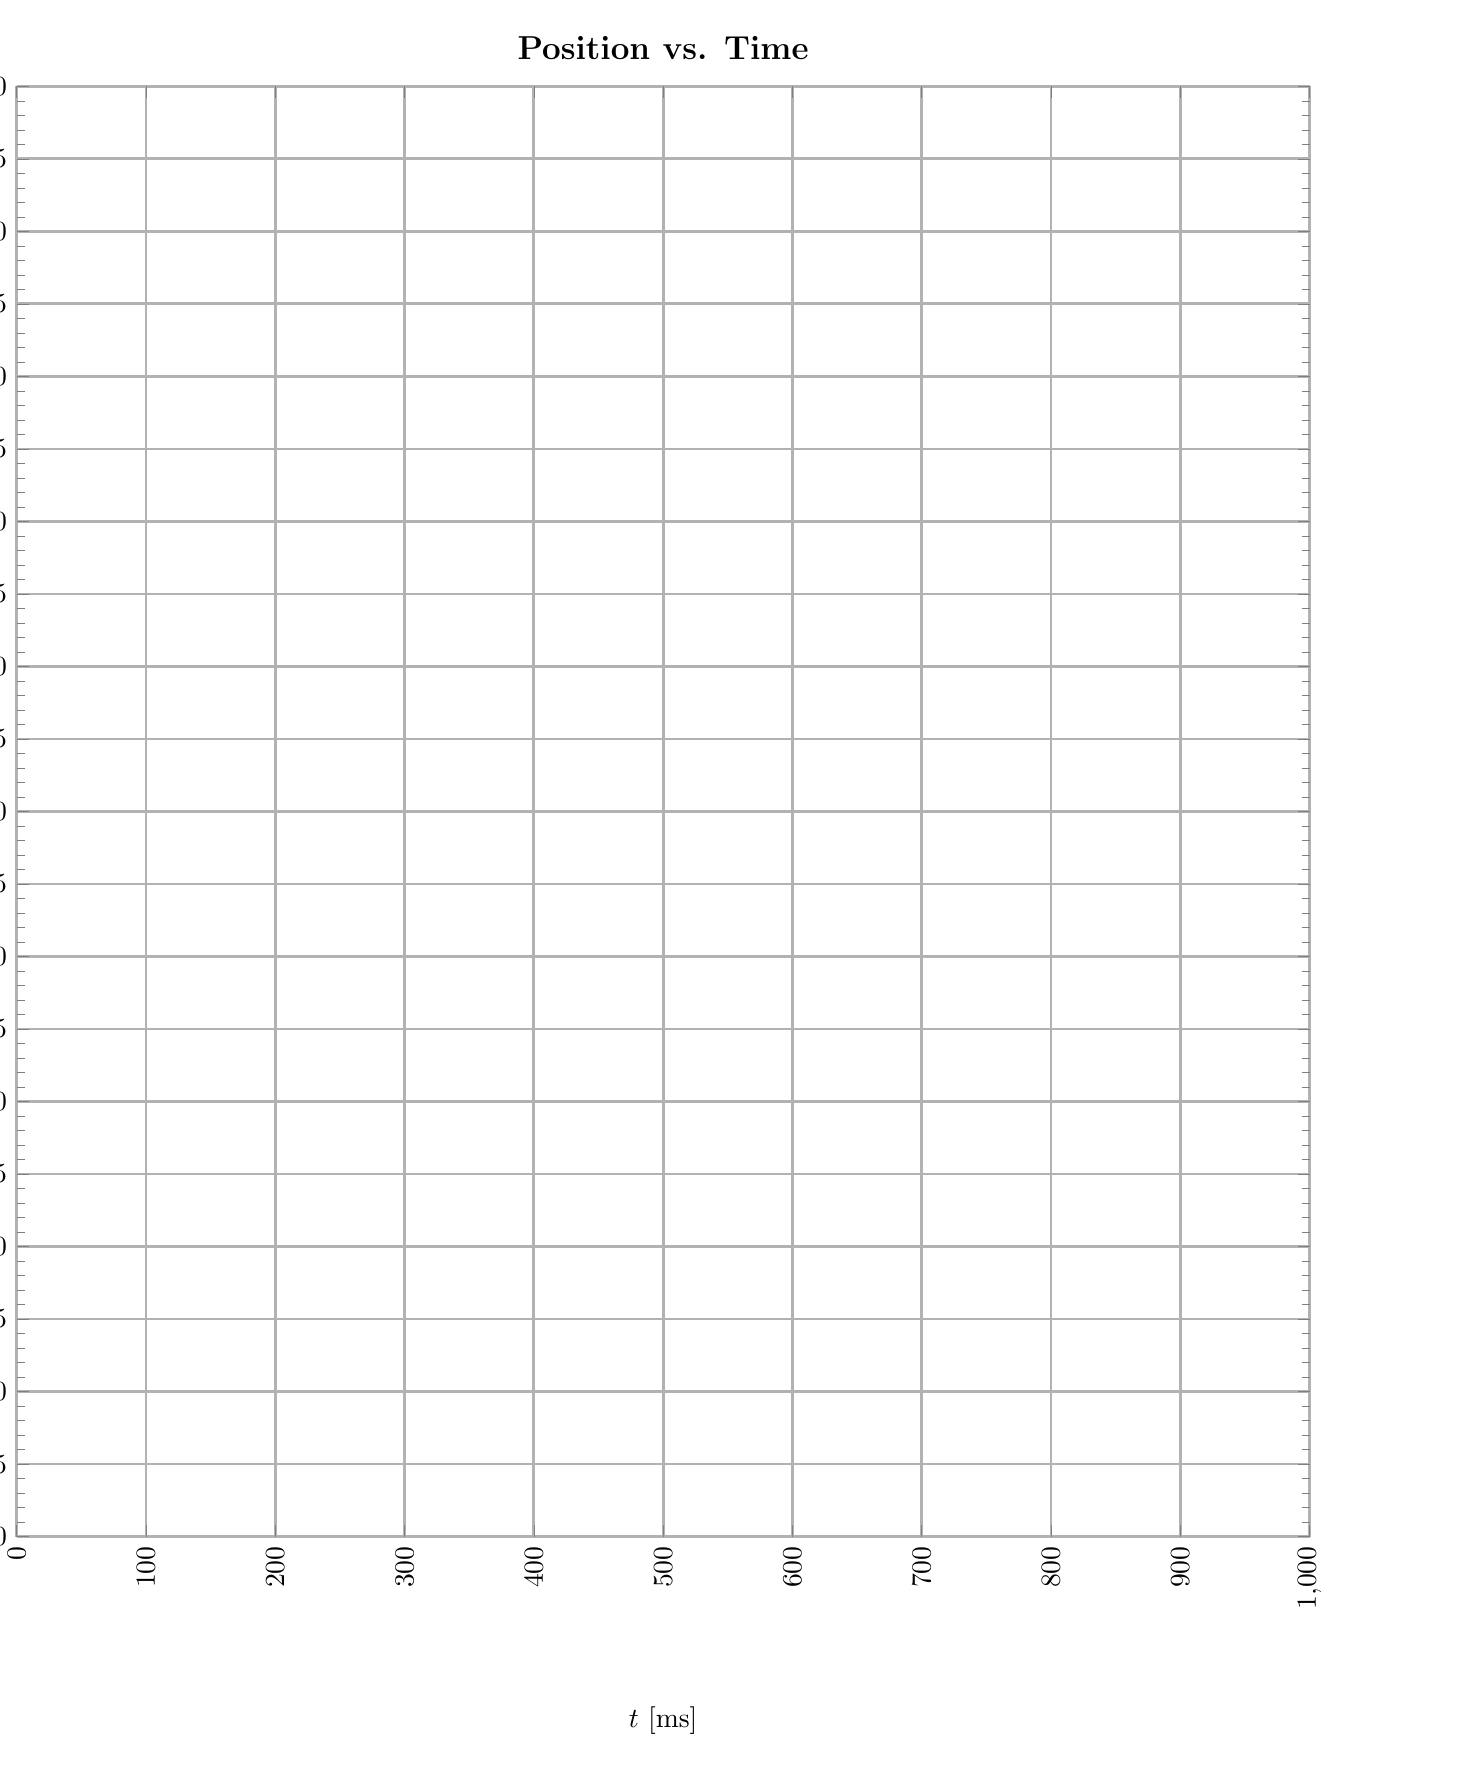
\begin{tikzpicture}
\hspace{-1.5cm}
\begin{axis}[
    title={\large\textbf{Position vs. Time}}, % Add a title here
    grid=major, % Add grid lines
    xlabel={$t$ [ms]}, % Label x-axis
    ylabel={$x(t)$ [cm]}, % Label y-axis
    xmin=0, xmax=1000, % X-axis range in seconds
    ymin=0, ymax=100, % Y-axis range in centimeters
    xtick={0, 100, ..., 1000}, % X-axis ticks every 0.1 seconds
    xticklabel style={rotate=90, anchor=near xticklabel},
    minor x tick num=0, % Disable x-axis subticks
    xlabel style={yshift=-1cm}, % Move the x-axis label down
    ytick={0, 5, ..., 100}, % Y-axis ticks every 10 cm
    % scaled x ticks=false, % Prevent scientific notation for x-axis tick labels
    minor y tick num=4, % Number of minor ticks between each major tick
    major grid style={line width=1pt,draw=gray!60},
    minor grid style={line width=1pt,draw=gray!60},
    axis line style={draw=none}, % Remove axis lines
    width=18cm, height=20cm, % Control size of the plot
]
\end{axis}
\end{tikzpicture}
\end{center}
\newpage
\question[2] Use the space below to plot your velocity (v) vs time (t) data: 

\begin{center}
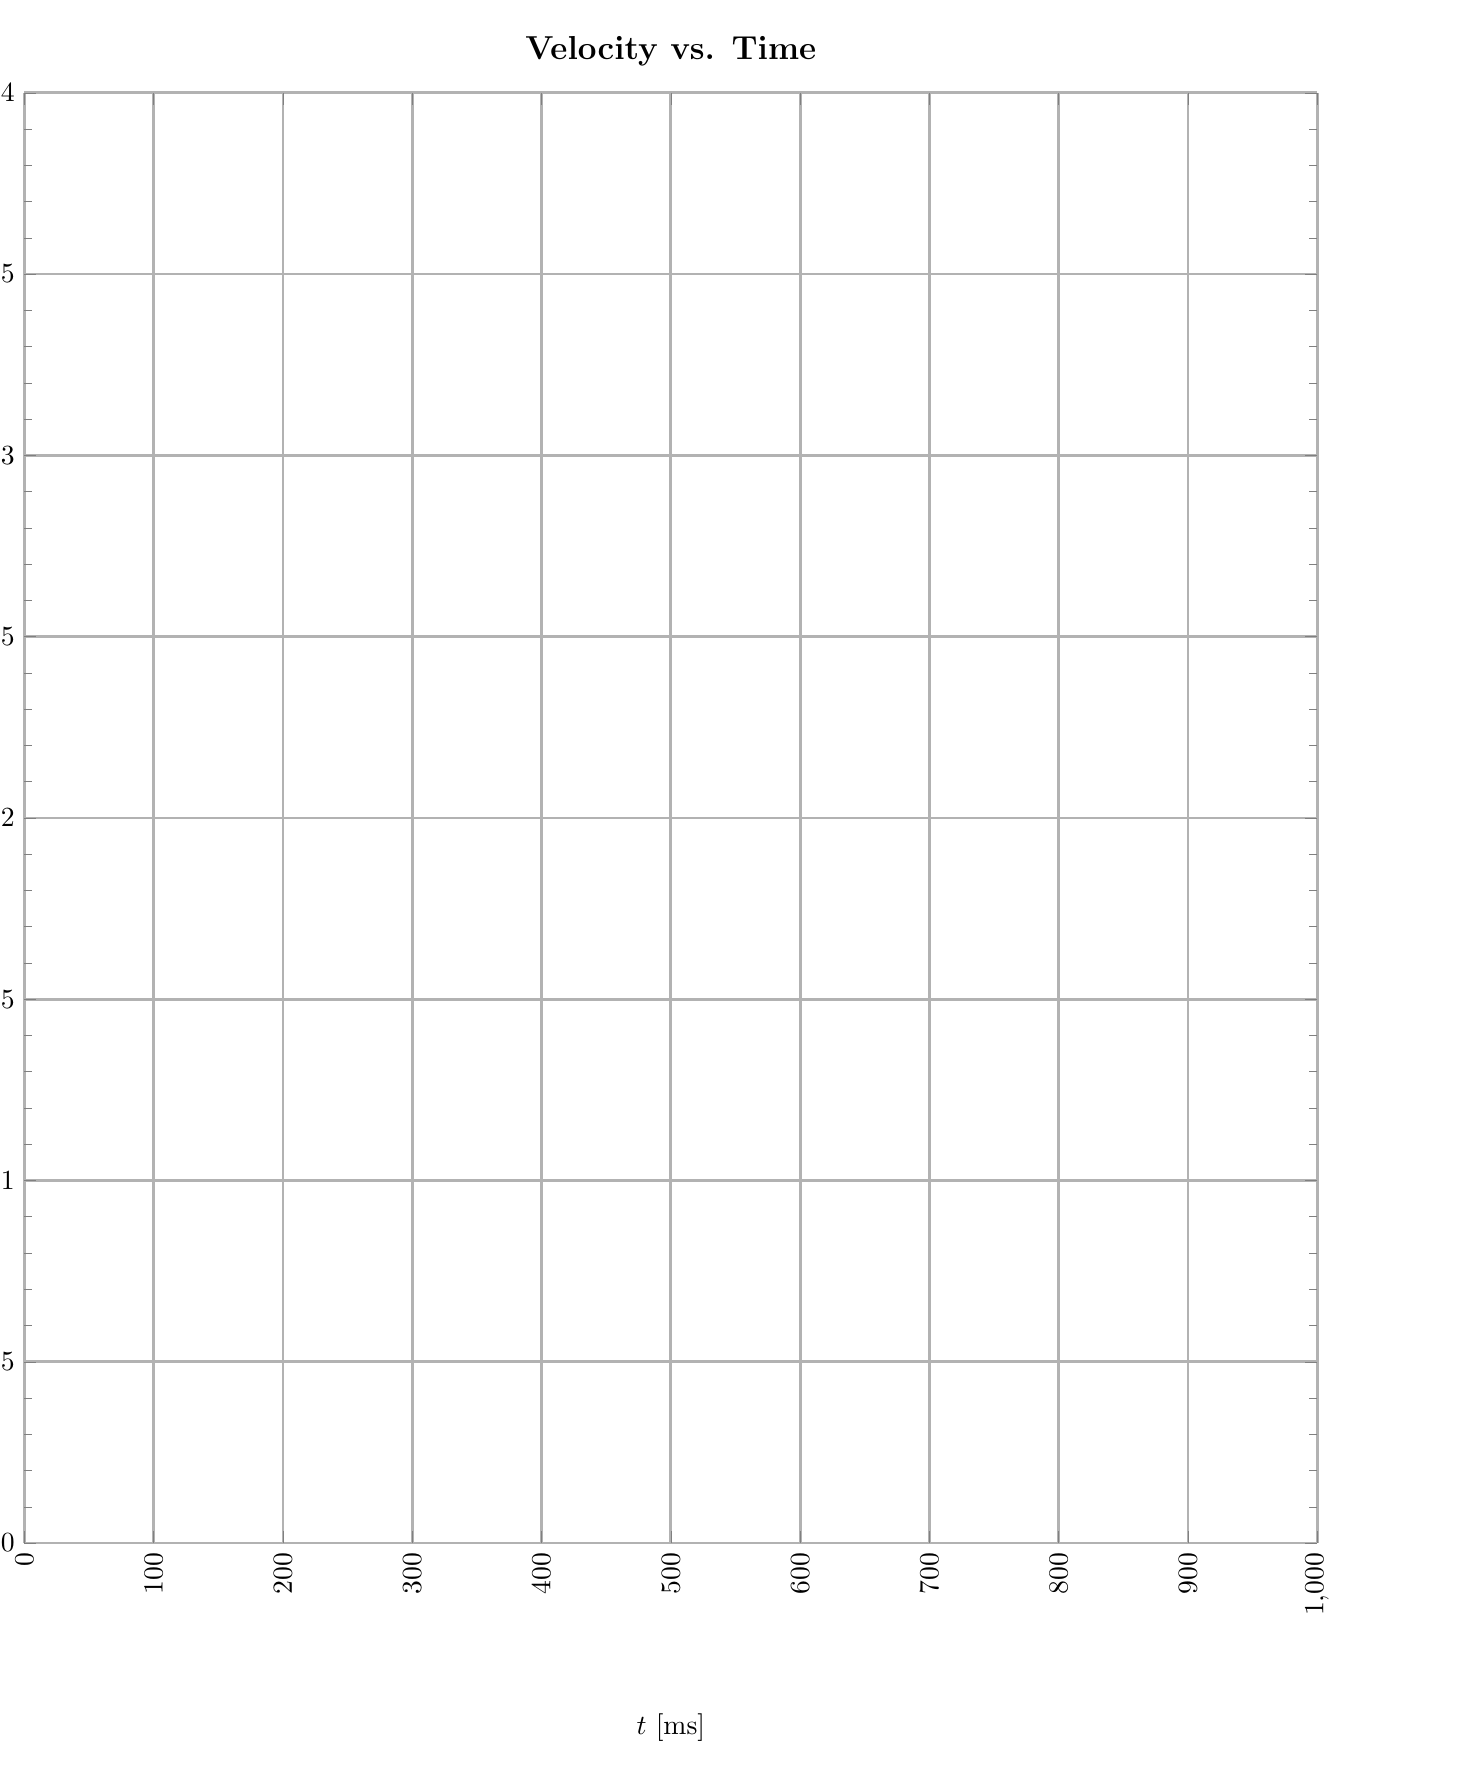
\begin{tikzpicture}
\hspace{-1.5cm}
\begin{axis}[
    title={\large\textbf{Velocity vs. Time}}, % Add a title here
    grid=major, % Add grid lines
    xlabel={$t$ [ms]}, % Label x-axis
    ylabel={$v(t)$ [cm/ms]}, % Label y-axis
    xmin=0, xmax=1000, % X-axis range in milliseconds
    ymin=0, ymax=0.4, % Y-axis range in cm/ms
    xtick={0, 100, ..., 1000}, % X-axis ticks every 100 ms
    xticklabel style={rotate=90, anchor=near xticklabel}, % Rotate x-axis tick labels
    minor x tick num=0, % Disable x-axis subticks
    xlabel style={yshift=-1cm}, % Move the x-axis label down
    ytick={0, 0.05,..., 0.4}, % Y-axis ticks every 0.05 cm/ms
    minor y tick num=4, % Number of minor ticks between each major tick for y-axis
    major grid style={line width=1pt, draw=gray!60}, % Style of major grid
    minor grid style={line width=1pt,draw=gray!60},
    axis line style={draw=none}, % Remove axis lines
    y tick label style={/pgf/number format/fixed, /pgf/number format/precision=2},
    width=18cm, height=20cm, % Control size of the plot
]

\end{axis}
\end{tikzpicture}
\end{center}

\qsp


\end{questions}
\end{document}
